\documentclass[10pt,a4paper]{article}
\usepackage[utf8]{inputenc}
\usepackage[english]{babel}
\usepackage{amsmath}
\usepackage{amsfonts}
\usepackage{amssymb}
\usepackage{hyperref}
\usepackage{graphicx}
\usepackage{caption}
\usepackage{subcaption}
\usepackage{color}
%
\graphicspath{ {../data/plots/} }
%
% \todo{} command.
% Usage: \todo{Document the TODO command.}
% Comment out second line to disable.
\newcommand{\todo}[1]{}
\renewcommand{\todo}[1]{{\color{red} TODO: {#1}} \\}
%
\newcommand{\AND}{\ensuremath{~AND~}}
\newcommand{\XOR}{\ensuremath{~XOR~}}
%
\author{Christian Bobach, 20104256}
\title{AMD tag overhead in a MPC outsourcing environment}
\begin{document}
\maketitle

\begin{abstract}
\todo{WRITE abstract}

\end{abstract}

\tableofcontents

%INTRODUCTION
%papers, problem, solutions, introduction to experiments
\section{Intorduction}
In this paper I have studied the paper \cite{fosc} and made experiments to mesure the overhed added to the computation by securing the input with an algebraic manipulation detection(AMD) code.

\todo{Introduction to paper \cite{fosc}}
In the paper they propose a framework for outsourcing secure multiparti computation(MPC) between any number of clients and workers with minimal overhead. The framework ensures input privacy is preserved and that the output is correct. This is done independant of the underlying MPC protocol. Their solusion minimize the work neede done by the client, while they try to minimize the overhead on the workers. For correctnes of output from the framework it is enough for one client to only trust one worker. This hes the effect hat the framework is not ensured to terminate as one worker can deadlock the system. They propose a way to detect a disonest worker and not to use that worker next time running the computation.

\todo{Introduction to problem and solution}
Because the workers has the possibility to add an error $\epsilon$ to the input of a client or before returning the result, there is a need for a tag to ensure the detection of such an addition. In the paper they propose usage of an AMD code to ensute that a worker cannot create an virable tag $\tilde{t}=Tag(\tilde{k},\tilde{x})$ where $\tilde{t}=t+\epsilon_t$, $\tilde{k}=k+\epsilon_k$ and $\tilde{x}=x+\epsilon_x$. If this is possible a corrupted worker could chose $\tilde{x}$ and creade a matching $\tilde{t}$ such that the protocol will not abort. This problem is exactly what the AMD code can overcome.

Then before the worekers output the secret shere of the function computed. They check that the entegrity of the tag is correct. A corrupted worker cannot change its share of the tag without breaking the security, and therby terminating the execution. This will reveal the corrupted worker and that will not be used in later computations. 

\todo{Introduction to experiment}
It is the overhead of the added tag that I have studied in this paper. In the paper they state that overhead is not big, but how big should the function computed be before the addition of the tag is negligabel. That is what I try to anwser in this paper.


%EXPERIMENT
%what have we covered
%what is the hypothesises
%what is the results
\section{Experiment}
The project was done using the duplo framework which is a framework for doing multiparti computations in a two parti setting. The framework is used to construct the two parties communicating in the experiments. The framework allows us to time the comunication. The two parties runs through six different phases during the execution. The six phases are setup, preprocess, solder, prepare, evaluate and decode. These phases give the possibility to time the computation in the different phases. After the six phases the parties hold their output computed based on their input and the circuit of the computation.

\todo{How was the experiemnts done}

The experiments in this paper is done using a composed circuit run through the framework. The experiemnt used two different composed circuit as inputs both of them consisting of multiple subcircuits. The first composed circuit we will call $C_{ITA}$ consists of an ID-, a TAG- and a variable number of AES-circuits. The other composed circuit we will call $C_{IA}$ consists of an ID-circuit and a variable number of AES-circuits. The TAG-circuit will be denoted $C_{T}$. In the framework used it is not possible to time the different subcircuits of the composed circuit. Therefore both $C_{ITA}$ and $C_{IA}$ is run multiple times to get an avarage of the execution time with and without $C_{T}$. From this we can get an estimate of how much time is used on the $C_{T}$ by calculating $C_{ITA}-C_{IA}$. When we have the time for the $C_{T}$ it is easy to get the fraction of the time is used on $C_{T}$ compared to the composed circuit by calculating $\frac{C_{T}}{C_{ITA}}$. This allow us to figure out how much time $C_{T}$ adds of overhead. Thereby we get an idea of how big a circuit should be before we can negiligate the overhead added by the AMD tag proposed in \cite{fosc}.

Before the expreiments could begin we needed the circuits that should be used. In the following sections I will introduce these circuits and why they were needed.

\subsection{Circuits}
The duplo framework had an AES-circuit that could be used as "the big computation", but we needed an ID- and a TAG-circuit before we could do the experiments. By "the big computation" is ment, a computation that could give an idea of when $C_{T}$ could be negligable. Here we use multiple AES circuits as the variable to see when this will happen. The ID-, TAG- and AES-circuit's would be soldere togeter to form the composed circuit that could be timed in the framework.

\bigskip
The input circuits are encoded using a slide modification of Nigel Smart's\footnote{Nighel's encoding can be found here: \url{https://www.cs.bris.ac.uk/Research/CryptographySecurity/MPC/}} circuit encoding. To generate the circuits I used a modifyed version of the Fariplay circuit generator tool\footnote{The circuit generator can be found here: \url{https://github.com/cbobach/circuit-generator}}.

\subsubsection{TAG-circuit}
The TAG circuit is made such that it forfills the requirements for the tag proposed in \cite{fosc}.

\todo{Security of the tag: do the math}
Such that the correctness of the output is guaranteed.

\todo{Description of tag circuit}
$C_T$ is constructed such that given 384 bit inputs from bothe patries, $x_1, k_1, s_1$ and $x_2, k_2, s_2$ where $x_i$ is the input to the calculation, $k_i$ is the key for the tag and $s_i$ is the seed where $|s_i|$ is the security parameter, for $i=1,2$. The tag is calculated as follows 

\begin{align*}
    Tag(x_1, k_1, s_1, x_2, k_2, s_2)
    &= 
    \begin{bmatrix}
        k_{1,1} & k_{2,1} & \dots & k_{1,128} & k_{2,128}    \\
        k_{1,2 }& k_{2,2} & \dots & s_{1,1}   & s_{2,1}      \\
        \vdots                                               \\
        s_{1,1} & s_{1,2} & \dots & s_{1,128} & s_{2,128}
    \end{bmatrix}
    \begin{bmatrix}
        x_{1,1}    \\
        x_{2,1}    \\
        \vdots     \\
        x_{1,128}  \\
        x_{2,128}
    \end{bmatrix}  \\
    &=
    \begin{bmatrix}
        x_{1,1}k_{1,1} + x_{2,1}k_{2,1} + \dots + x_{1,128}k_{1,128} + x_{2,128}k_{2,128}    \\
        x_{1,1}k_{1,2} + x_{2,1}k_{2,2} + \dots + x_{1,128}s_{1,1} + x_{2,128}s_{2,1}      \\
        \vdots \\
        x_{1,1}s_{1,1} + x_{2,1}s_{2,1} + \dots + x_{1,128}s_{1,128} + x_{2,128}s_{2,128}        
    \end{bmatrix}    \\
    &= 
    \begin{bmatrix}
        t_0    \\
        \vdots    \\
        t_{128}
    \end{bmatrix}
\end{align*}

This calculation was converted into a circuit such that if $k'_i= k_i||s_i$ and$t'_{i,j,l} = x_{i,l} \AND k'_{i,l+j}$ then $t_j = t'_{1,j,1} \XOR t'_{2,j,1} \XOR \dots \XOR t'_{1,j,128} \XOR t'_{2,j,128}$, for $i=1,2$, $j=0,\dots, 128$ and $l=1,\dots, 128$. Since $\AND$ has the structore of multiplication in binary and $\XOR$ the structure of addition, as can be seen in table \ref{and xor gates}.

\begin{table}[h]
    \begin{subtable}{.5\linewidth}
    \centering
    \begin{tabular}{l l || l}
        l-wire & r-wire & l $\AND$ r    \\\hline
        0 & 0 & 0    \\
        0 & 1 & 0    \\
        1 & 0 & 0    \\
        1 & 1 & 1    
    \end{tabular}
    \caption{$\AND$-gate}
    \end{subtable}%
    \begin{subtable}{.5\linewidth}
    \centering
    \begin{tabular}{l l || l}
        l-wire & r-wire & l $\XOR$ r    \\\hline
        0 & 0 & 0    \\
        0 & 1 & 1    \\
        1 & 0 & 1    \\
        1 & 1 & 0    
    \end{tabular}
    \caption{$\XOR$-gate}
    \end{subtable} 
\caption{Logical gates }
\label{and xor gates}
\end{table}

Constructiong the circuit like this result in a circuit with 768 input and 129 output
wires. Internal $C_T$ consist of 66687 wires and 65919 gates where 33024 of these gates are the expensive $\AND$ gates. No optimization has been done to reduce the numer of $\AND$ gates in the circuit.

\subsubsection{ID-circuit}
The ID-circuit was needed since the framework did not support that the inputwires of the composed circuit could go to multiple subcircuits. Therefor we needed a input circuit that could overcome this. Because of the construction of the framework a subcircuit needed to consist of bothe gates and wires.

\bigskip
The ID-circuit, denoted $C_{I}$ is a circuit where the input and output are the same. Because a subcircuit needed to have gates it was first constructed by using two layers of $NAND$-gates. This was later optimized to use one layer of $AND$ gates instead. This was done by takes each input wire and $AND$ it with itself to get the same output as input which is ilustraded by table \ref{and xor gates}.

Since the input of the composed circuit is based on the input of $C_A$, the key size and the security parameter of $C_T$. The number of input wires to $C_I$ is the same as $C_{ITA}$. As we use 128 bit AES and 128 bit as key and security parameter $C_I$ has 768 inputwires in total, 384 from each parti. This gives us an additionl 768 $AND$-gates and 1536 wires that $C_I$ adds to the composed circuit. 


\subsubsection{Soldering}
\todo{Description of the soldering phase: parallel, input to output}
In each run of the two parti computation the different circuits is soldered together to cunstruct the composed circuit. Since aes is used as the computation of the experiment then input frm the two parties shouls be maped correctly at the same time we had the tag circuit that uses the complete input. The composed circuit sonsist of two layers of circuits. In the first layer we have $C_I$ such that we have the same output of layer one as input. In the second layer we have $C_T$ as the first circuit. This circuit uses the complete output from $C_I$ as input and output the tag vektor. The rest of the circuits of the second layer consist of $C_A$'s ranging from 0 and upwards, such that they are soldered to $C_I$ in parallel. Since the $C_A$'s does not use the complete output from $C_I$ the correct output wires need to be soldered to the correct inputwires of the $C_A$'s. As the input to $C_A$ is the first 128 bit outputwires from both parties in $C_I$ thise should be soldered to the such that the outputwires 0 to 127 and 384 to 511 are used as input to each of the $C_A$'s. By soldering multiple $C_A$'s in to the composed circuit we obtain a bigger circuit. That we can use to mesure the tag overhead.

For the framework to work it is important to keep track of which wire indexes goes to which circuit an wich indexes should be on the new outputwires. This can be found in the source code for the duplo framework found in the repository for this project.\footnote{Code for this experiment can be found on github here: \url{https://github.com/cbobach/mpc-outsourcing}} The code relevant for the soldering of circuits is found in the header file.

\subsection{Results}
In this section I will try to explain what we can see from the timing of the different phases when running the composed circuit in the framework. All the results can be found in appendix \ref{data appendix}. In the following section will I only include the plots that are interresting.

First of all we can eliminte the setup phase, since that does not dependant on the circuit but is a technical phase were the parties are prepared. So the first interristing phase to look at is the preprocess phase.

%PREPROCESS
\begin{figure}[h]
    \centering
    \begin{subfigure}[t]{0.3\textwidth}
        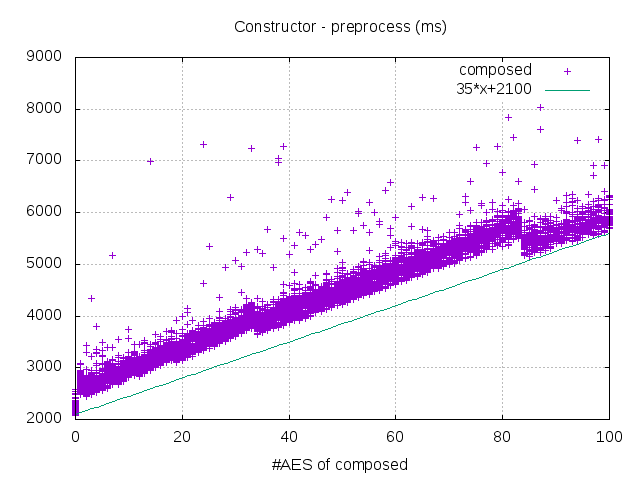
\includegraphics[width=\textwidth]{const_preprocess_plots}
        \caption{}
        \label{preprocess composed}
    \end{subfigure}
    \begin{subfigure}[t]{0.3\textwidth}
        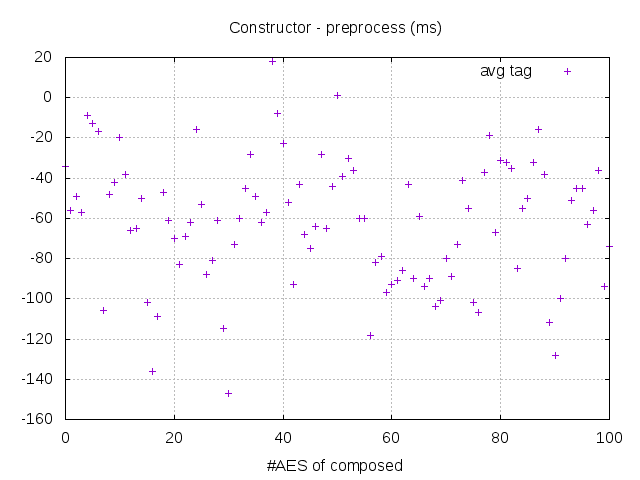
\includegraphics[width=\textwidth]{const_preprocess_avg}
        \caption{}
        \label{preprocess tag}
    \end{subfigure}
    \begin{subfigure}[t]{0.3\textwidth}
        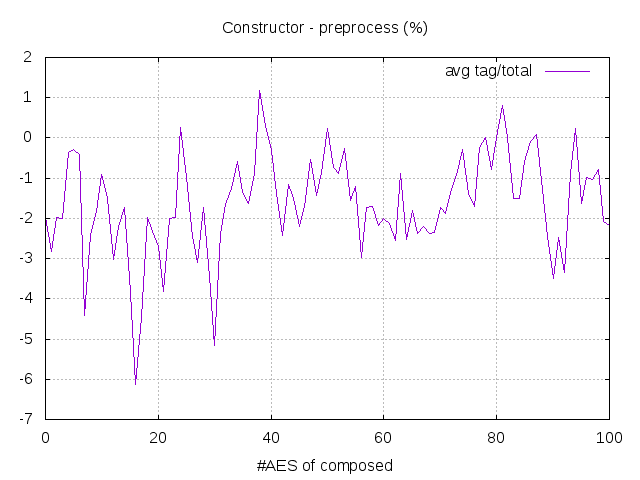
\includegraphics[width=\textwidth]{const_preprocess_frac}
        \caption{}
        \label{preprocess frac}
    \end{subfigure}
    \caption{The preprocess phase}
\end{figure}

In figure \ref{preprocess composed} we see that the preprocessing time of the composed circuit looks linear to de number of AES subcircuits. We also see that the total time used preprocessing starts around 2-3 seconds without any AES subcircuits and goes up to between 6 to 7 seconds with 100 AES subcircuits. 
Looking at figure \ref{preprocess tag} we see that for the most plot is less then 0. This implies that the tag part of the circuit is such small that it is not mesurable. 
At figure \ref{preprocess frac} we also see that the fraction of time used preprocessing the tag part of the circuit is minimal and belove 1\%.

%SOLDER
\begin{figure}[h]
    \centering
    \begin{subfigure}[t]{0.3\textwidth}
        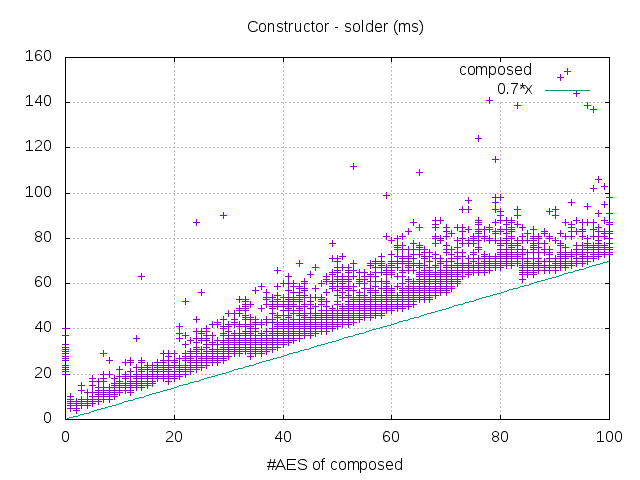
\includegraphics[width=\textwidth]{const_solder_plots}
        \caption{}
        \label{solder composed const}
    \end{subfigure}
    \begin{subfigure}[t]{0.3\textwidth}
        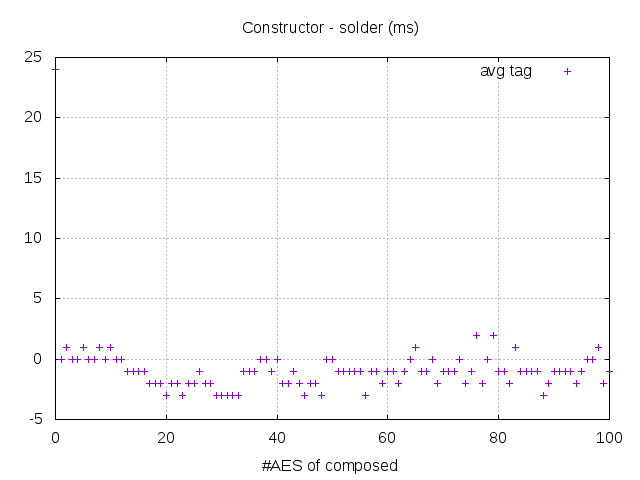
\includegraphics[width=\textwidth]{const_solder_avg}
        \caption{}
        \label{solder tag const}
    \end{subfigure}
    \begin{subfigure}[t]{0.3\textwidth}
        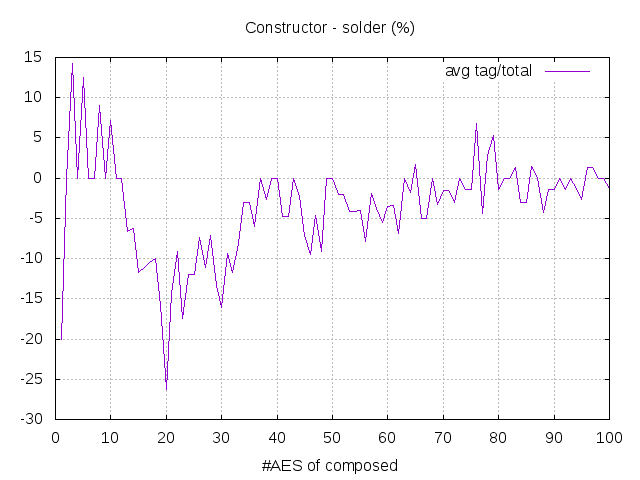
\includegraphics[width=\textwidth]{const_solder_frac}
        \caption{}
        \label{solder frac const}
    \end{subfigure}

    \begin{subfigure}[t]{0.3\textwidth}
        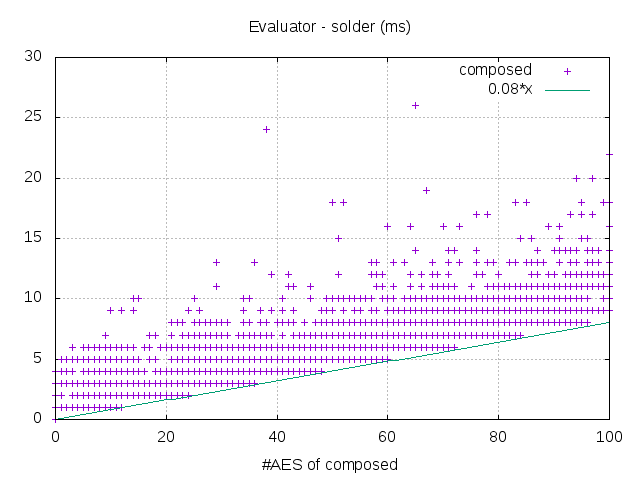
\includegraphics[width=\textwidth]{eval_solder_plots}
        \caption{}
        \label{solder composed eval}
    \end{subfigure}
    \begin{subfigure}[t]{0.3\textwidth}
        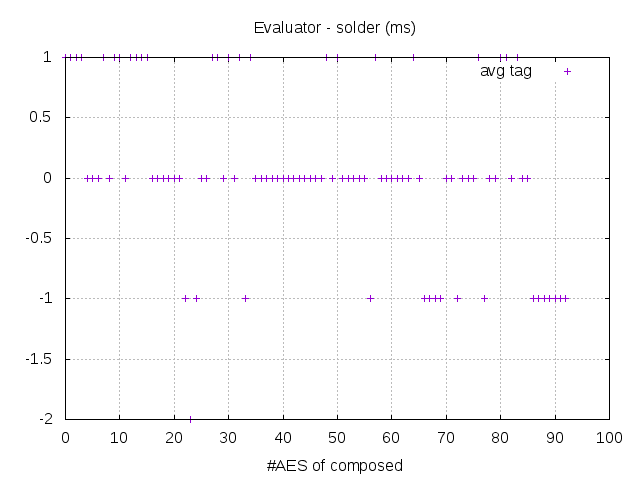
\includegraphics[width=\textwidth]{eval_solder_avg}
        \caption{}
        \label{solder tag eval}
    \end{subfigure}
    \begin{subfigure}[t]{0.3\textwidth}
        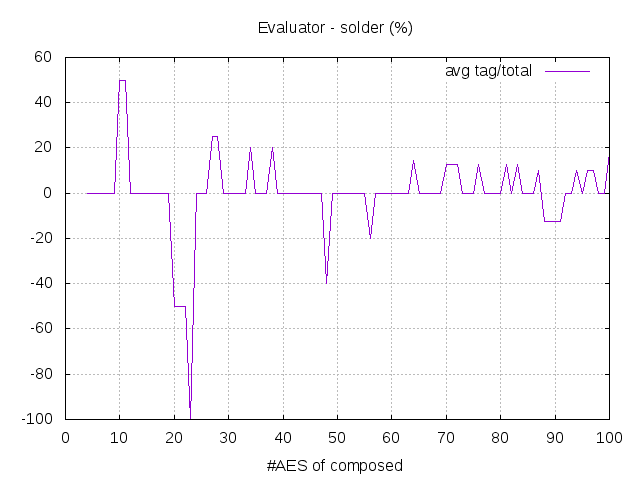
\includegraphics[width=\textwidth]{eval_solder_frac}
        \caption{}
        \label{solder frac eval}
    \end{subfigure}
    \caption{The soldering phase}
\end{figure}

In the solder phase of the execution we see a difference between the two parties. In the figure we see that both \ref{solder composed const} and \ref{solder composed eval} are lineare encreasing. It looks like there is a factor 10 in difference in the slope between them. Then looking at the average time used on the tag in the plots \ref{solder tag const} and \ref{solder tag eval} we see that this looks like a constant less than 1. Which gives us a fraction as seen in \ref{solder frac const} and \ref{solder frac eval} is decreasing on the spikes and over the number of AES circuits in the composed is going towards something negligable.

%PREPARE
\begin{figure}[h]
    \centering
    \begin{subfigure}[t]{0.3\textwidth}
        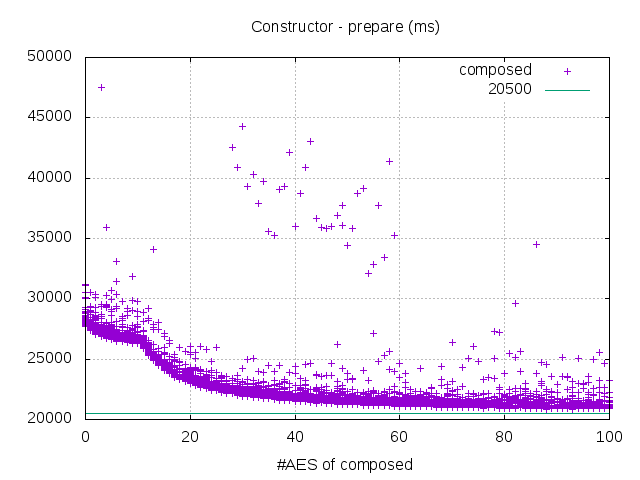
\includegraphics[width=\textwidth]{const_prepare_plots}
        \caption{}
        \label{prepare composed}
    \end{subfigure}
    \begin{subfigure}[t]{0.3\textwidth}
        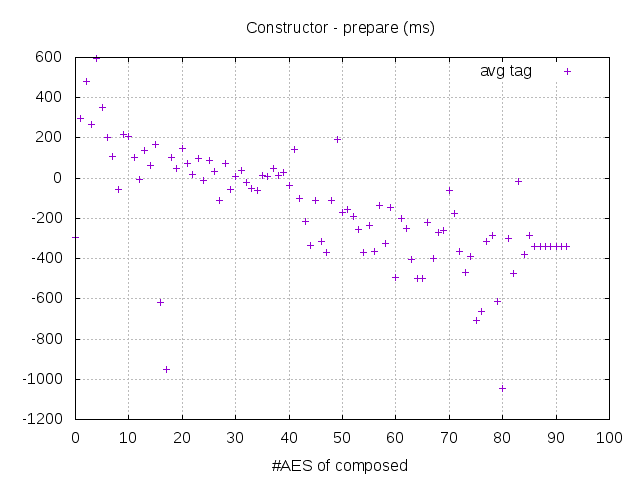
\includegraphics[width=\textwidth]{const_prepare_avg}
        \caption{}
        \label{prepare tag}
    \end{subfigure}
    \begin{subfigure}[t]{0.3\textwidth}
        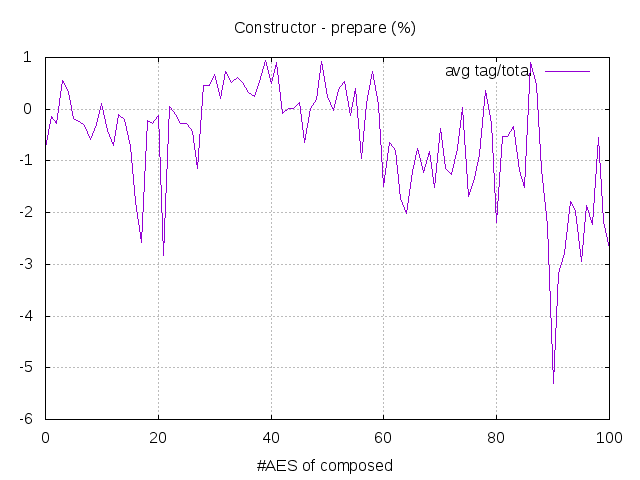
\includegraphics[width=\textwidth]{const_prepare_frac}
        \caption{}
        \label{prepare frac}
    \end{subfigure}
    \caption{The prepare phase}
\end{figure}

In the prepare phase the two parties plots are close to equivalente. This time we see that the time used on the composed circuit in figure \ref{prepare composed} is decreasing and it looks like it is going towards a constant around 20 seconds. This is because the framework is optimized to work on big circuits.
Loking at the plots for the average time in figure \ref{prepare tag} we see that all the plots are belowe 200 ms, and maybe the average is decreasing slightly. But in worst case it is a constant less than the 200 ms.

This results in a fraction of time used on the circuit that is in worst case is constant, bu looking at the figure \ref{prepare frac} it looks like it might be decreasing. But one again we see that many parts of the graph is belove 0 which tells us that the time used on the tag part is small compared to the time used on the total composed circuit. We see that the fraction is less then 1\% of the total.

%EVALUATE
\begin{figure}[h]
    \centering
    \begin{subfigure}[t]{0.3\textwidth}
        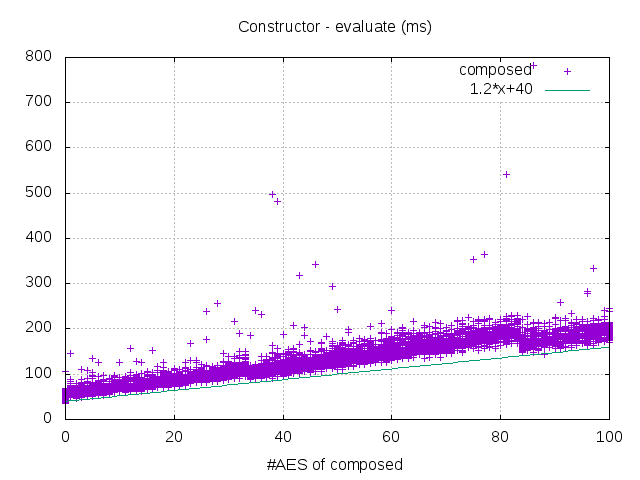
\includegraphics[width=\textwidth]{const_eval_plots}
        \caption{}
        \label{eval composed}
    \end{subfigure}
    \begin{subfigure}[t]{0.3\textwidth}
        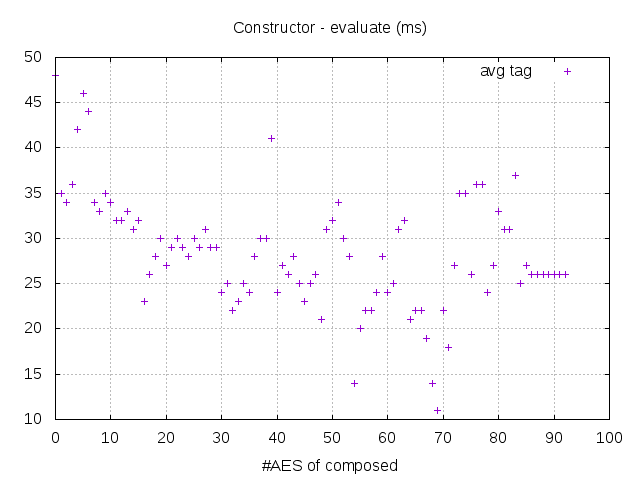
\includegraphics[width=\textwidth]{const_eval_avg}
        \caption{}
        \label{eval tag}
    \end{subfigure}
    \begin{subfigure}[t]{0.3\textwidth}
        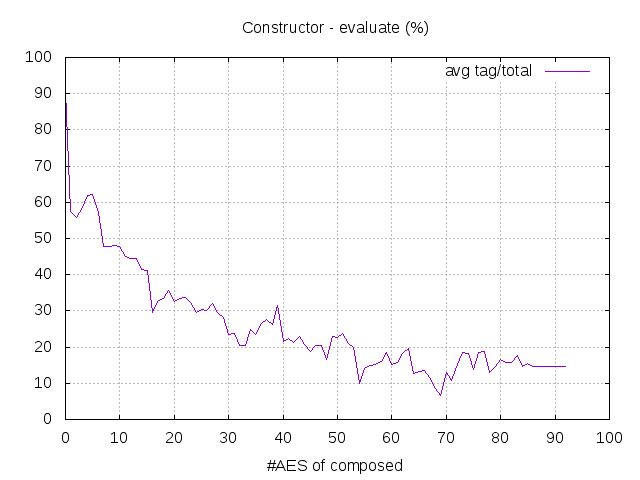
\includegraphics[width=\textwidth]{const_eval_frac}
        \caption{}
        \label{eval frac}
    \end{subfigure}
    \caption{The evaluation phase}
\end{figure}

Once again the two parties are similar when looking at the plots. This time again we see that the time used on the composed circuit is linear encreasing in the evaluation phase in figure \ref{eval composed}. When we look at the average time used on the tag in figure \ref{eval tag} we see that it looks like it is linear and slightly decreasing. This results in the fraction we see in figure \ref{eval frac}. Here it is clearly that the fraction of time used on the tag part is decreasing and it looks like it is approximating a constant that is around 10\% of the composed circuit.

%DECODE
\begin{figure}[h]
    \centering
    \begin{subfigure}[t]{0.3\textwidth}
        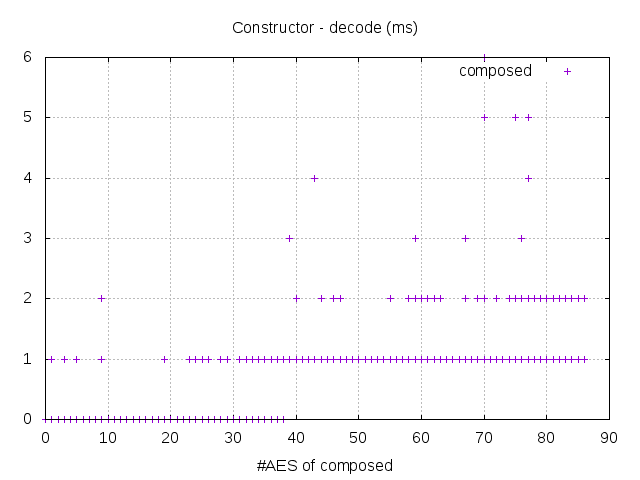
\includegraphics[width=\textwidth]{const_decode_plots}
        \caption{}
        \label{decode composed const}
    \end{subfigure}
    \begin{subfigure}[t]{0.3\textwidth}
        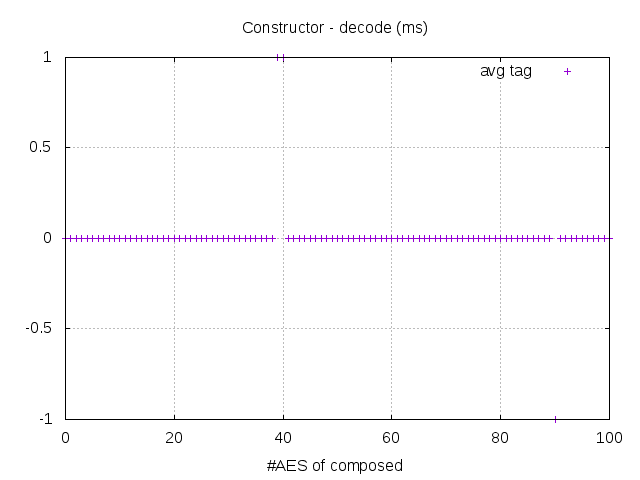
\includegraphics[width=\textwidth]{const_decode_avg}
        \caption{}
        \label{decode tag const}
    \end{subfigure}
    \begin{subfigure}[t]{0.3\textwidth}
        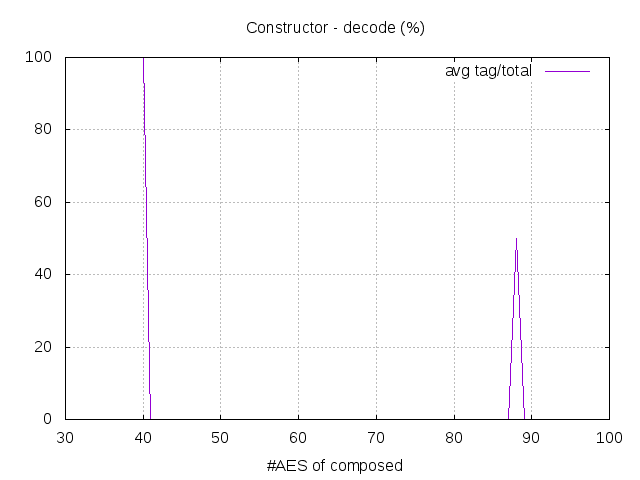
\includegraphics[width=\textwidth]{const_decode_frac}
        \caption{}
        \label{decode frac const}
    \end{subfigure}

    \begin{subfigure}[t]{0.3\textwidth}
        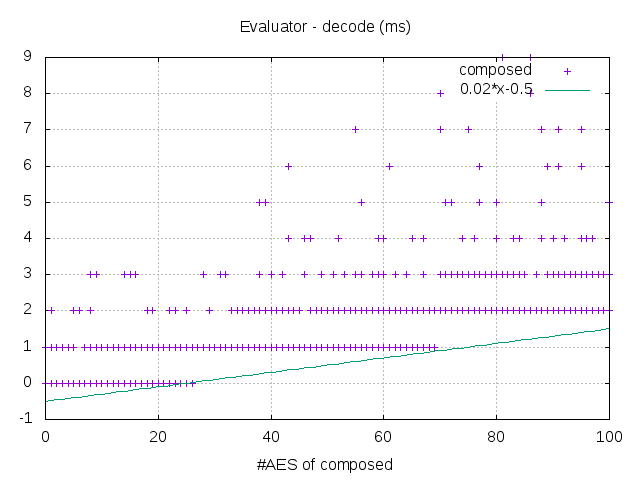
\includegraphics[width=\textwidth]{eval_decode_plots}
        \caption{}
        \label{decode composed eval}
    \end{subfigure}
    \begin{subfigure}[t]{0.3\textwidth}
        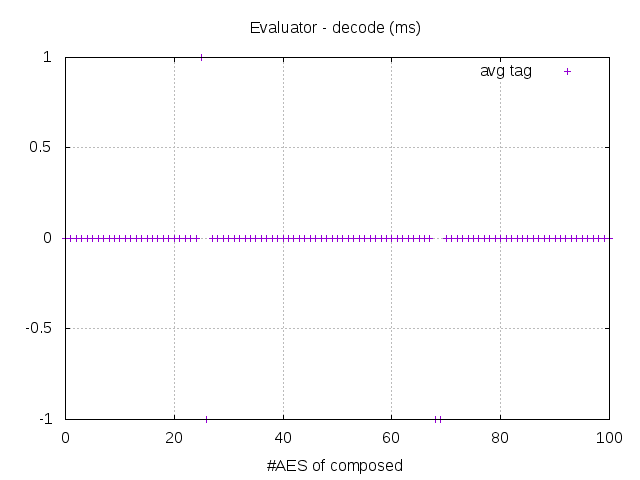
\includegraphics[width=\textwidth]{eval_decode_avg}
        \caption{}
        \label{decode tag eval}
    \end{subfigure}
    \begin{subfigure}[t]{0.3\textwidth}
        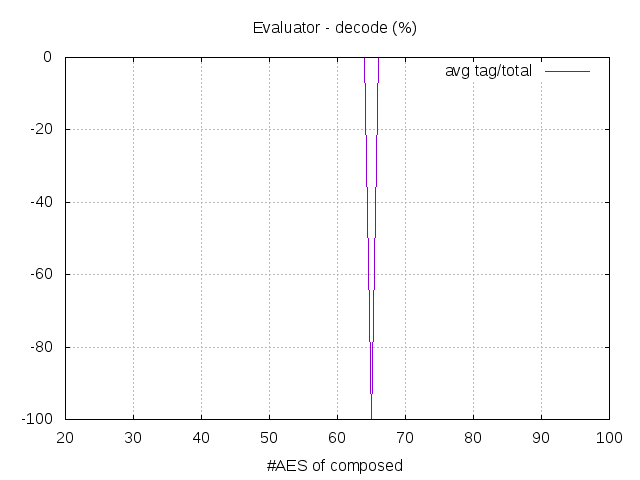
\includegraphics[width=\textwidth]{eval_decode_frac}
        \caption{}
        \label{decode frac eval}
    \end{subfigure}
    \caption{The decode phase}
\end{figure}

\todo{Describe the decode phase}
In the decode phase we do not see the exact same resulta at both parties. But in general it looks like the plots in both \ref{decode composed const} and \ref{decode composed eval} are linear encreasing. From \ref{decode tag const} and \ref{decode tag eval} we see that the average time used on the tag part is constant and negligable. The same goes for the fraction, as seen in \ref{decode frac const} and \ref{decode frac eval}.

\todo{Describe the overall results, total}
\bigskip
Summing this up to calculate a fraction of the time used on the tag pat of the composed circuit depandant on the number of AES circuits. We get the firure \ref{total frac} which shows that as an upper bound that the tag part of the composed circuit is approcing 0 as the amount of AES circuits encreases.

\begin{figure}[h]
    \centering
    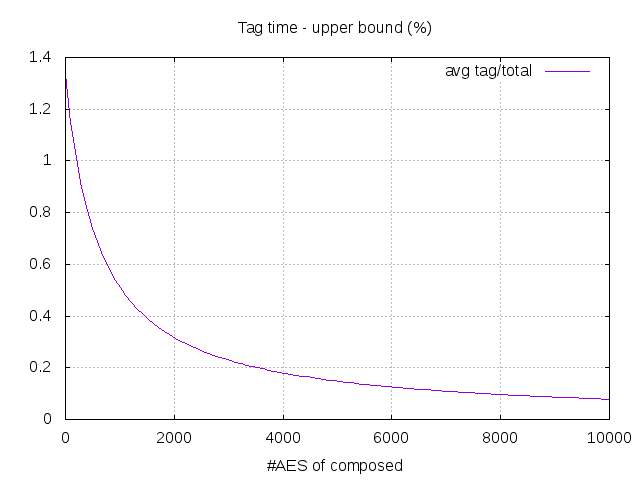
\includegraphics[width=0.5\textwidth]{total_frac}
    \caption{Total tag fraction of composed, $\frac{300}{36x+22500}$}
    \label{total frac}
\end{figure}


\subsection{Discussion}
%DISCUSSION - optimizing results
\todo{Using laptop}
\todo{Problems with this way of timing}
\todo{Optimization on statistics}


%CONCLUTION
\section{Conclution}
\todo{What was the hypothesis}
\todo{What was the conclution}

%CONTINIUED WORK
%proposals for further work
\section{Continiued work}
\todo{Are the more work to be done?}

\pagebreak

%BIB
\bibliography{report}
\bibliographystyle{alpha}

\appendix

\section{Data}
\label{data appendix}
All data generated and used in this report can be found at \href{https://github.com/cbobach/mpc-outsourcing}{github}\footnote{All the data files and plots can be found here: https://github.com/cbobach/mpc-outsourcing}. The data was generated using a framework 'duplo' which is an ongoing phd. project by Roberto Trifiletti, which is not public at the moment of writing. All data was collected via a localhost on a standard laptop with a i5-4210U, 1.7GHz processor, 12Gb 1600MHz ram and 6.0Gb/s ssd running Ubuntu 16.10.

The framewok conist of 6 different phases, setup, preprocess, solder, prepare, evaluate and decode. Each of these except setup timed are plottet in the following figures. Each of the subsections contins six polots, the first three are form the constructor and the next three are from the evaluator.

For conclution on the different plots and the hypothesis can be read in the abstract and conclution.

\begin{figure}[h]
    \centering
    \begin{subfigure}[t]{0.3\textwidth}
        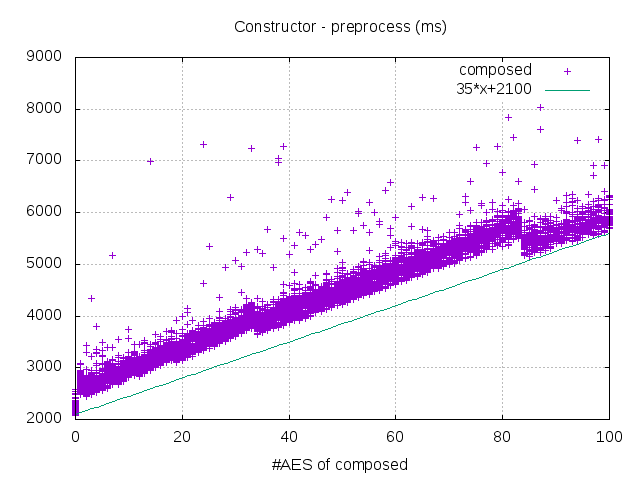
\includegraphics[width=\textwidth]{const_preprocess_plots}
        \caption{Constructor, total time used on the composed circuit}
    \end{subfigure}
    \begin{subfigure}[t]{0.3\textwidth}
        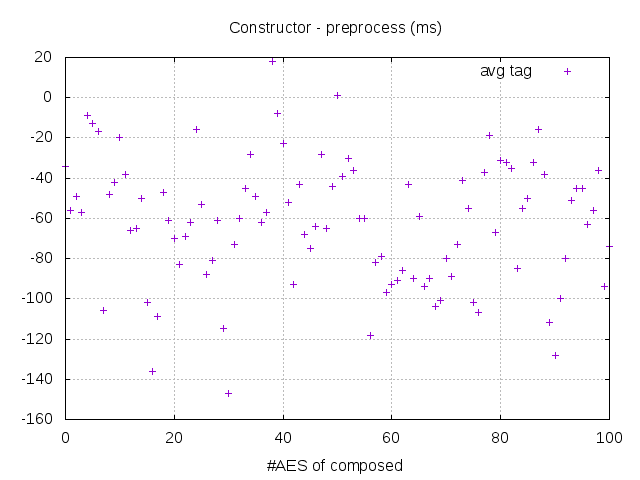
\includegraphics[width=\textwidth]{const_preprocess_avg}
        \caption{Constructor, average time used on tag part}
    \end{subfigure}
    \begin{subfigure}[t]{0.3\textwidth}
        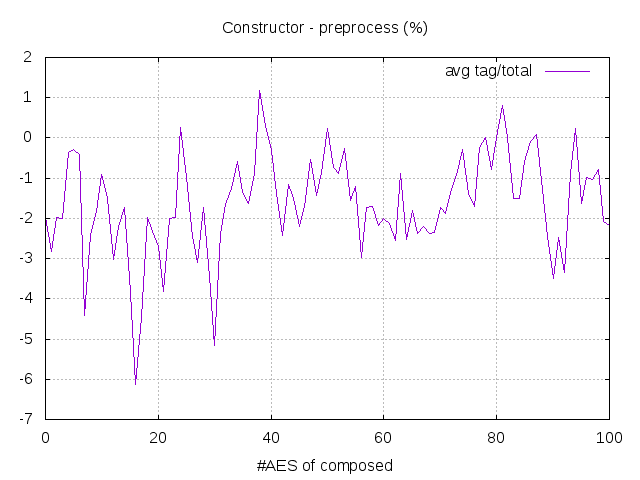
\includegraphics[width=\textwidth]{const_preprocess_frac}
        \caption{Constructor, fraction of time used on tag part}
    \end{subfigure}

    \begin{subfigure}[t]{0.3\textwidth}
        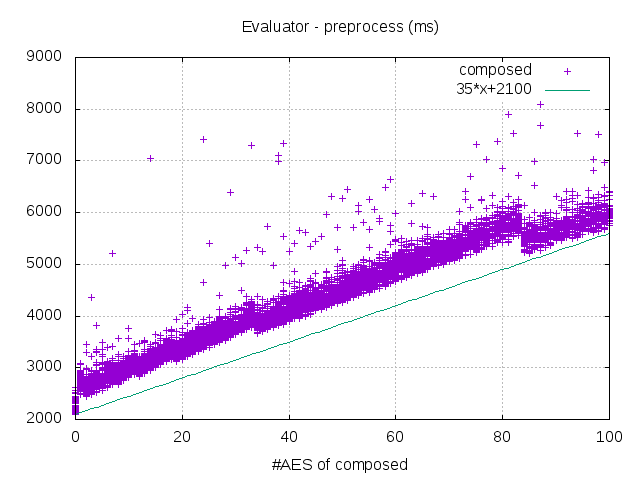
\includegraphics[width=\textwidth]{eval_preprocess_plots}
        \caption{Evaluator, total time used on the composed circuit}
    \end{subfigure}
    \begin{subfigure}[t]{0.3\textwidth}
        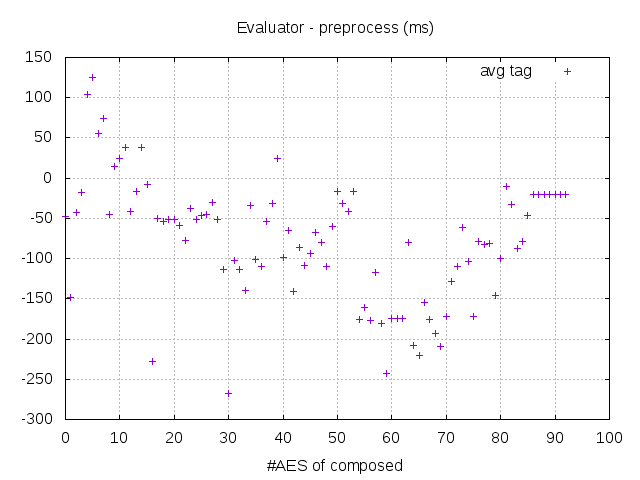
\includegraphics[width=\textwidth]{eval_preprocess_avg}
        \caption{Evaluator, average time used on tag part}
    \end{subfigure}
    \begin{subfigure}[t]{0.3\textwidth}
        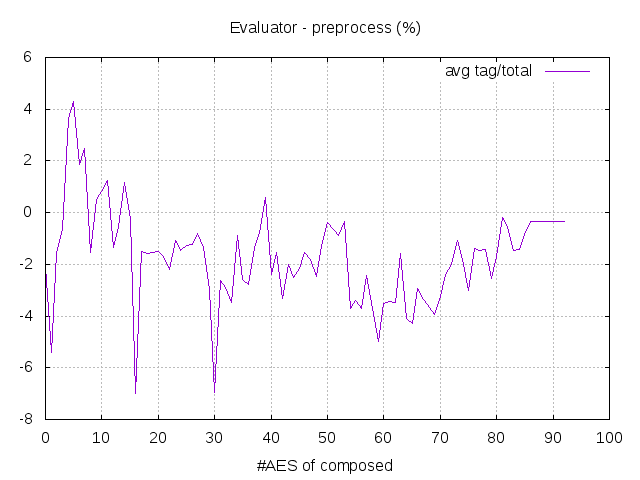
\includegraphics[width=\textwidth]{eval_preprocess_frac}
        \caption{Evaluator, fraction of time used on tag part}
    \end{subfigure}
    \caption{The preprocess phase is run on one instance of the ID- and TAG-circuit, while it is run on multiple instances of the AES-circuit.}
    \label{data preprocess}
\end{figure}

\begin{figure}[h]
    \centering
    \begin{subfigure}[t]{0.3\textwidth}
        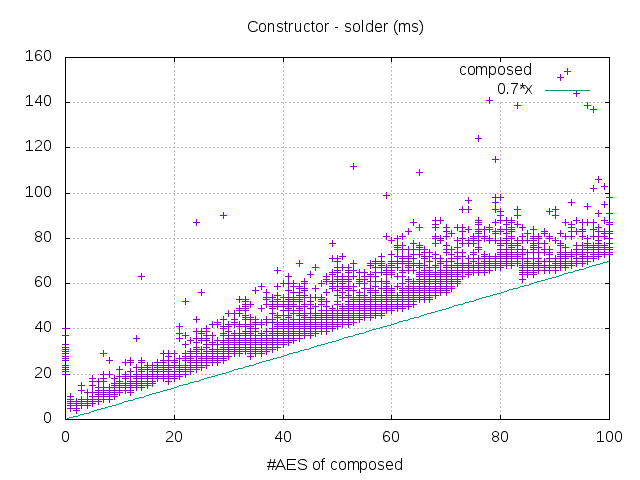
\includegraphics[width=\textwidth]{const_solder_plots}
        \caption{Constructor, total time used on the composed circuit}
    \end{subfigure}
    \begin{subfigure}[t]{0.3\textwidth}
        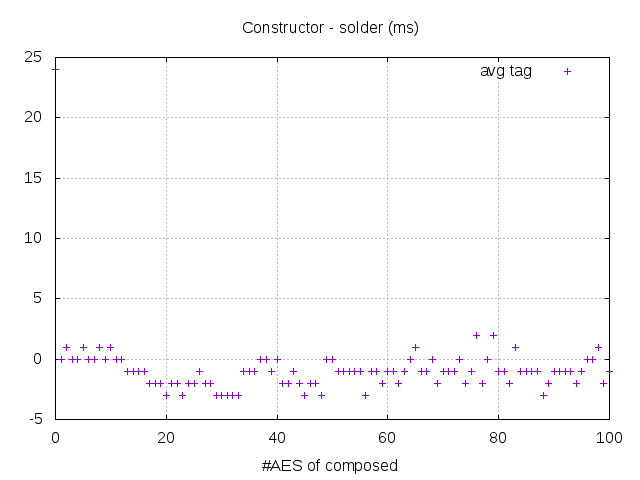
\includegraphics[width=\textwidth]{const_solder_avg}
        \caption{Constructor, average time used on tag part}
    \end{subfigure}
    \begin{subfigure}[t]{0.3\textwidth}
        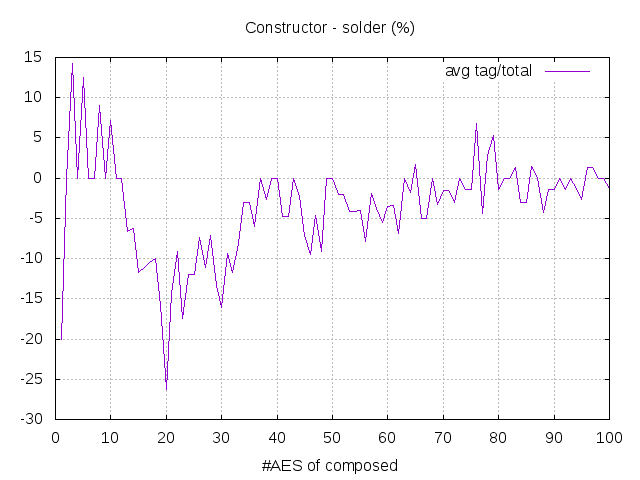
\includegraphics[width=\textwidth]{const_solder_frac}
        \caption{Constructor, fraction of time used on tag part}
    \end{subfigure}

    \begin{subfigure}[t]{0.3\textwidth}
        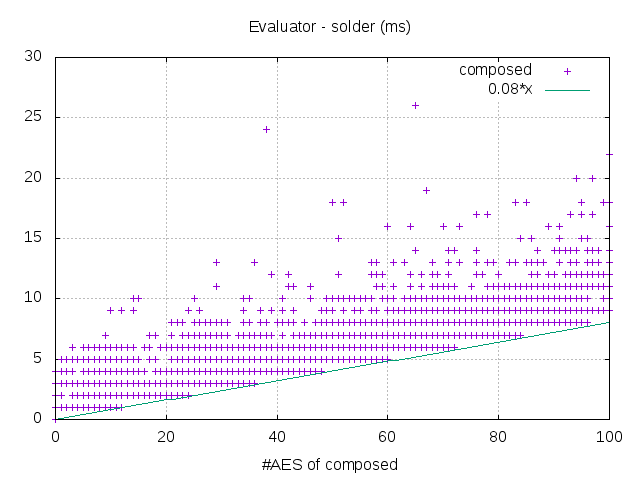
\includegraphics[width=\textwidth]{eval_solder_plots}
        \caption{Evaluator, total time used on the composed circuit}
    \end{subfigure}
    \begin{subfigure}[t]{0.3\textwidth}
        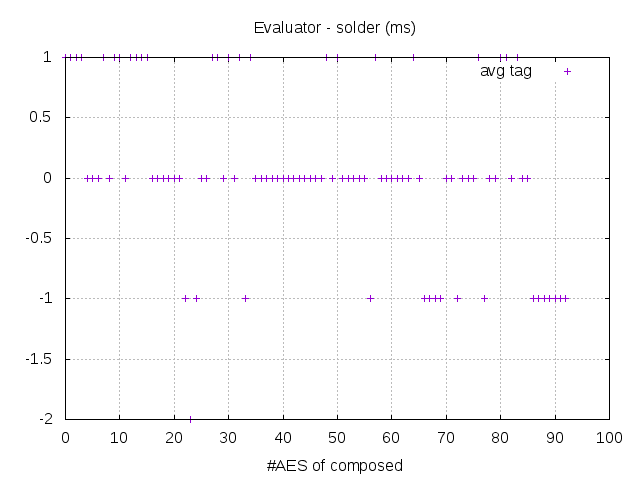
\includegraphics[width=\textwidth]{eval_solder_avg}
        \caption{Evaluator, average time used on tag part}
    \end{subfigure}
    \begin{subfigure}[t]{0.3\textwidth}
        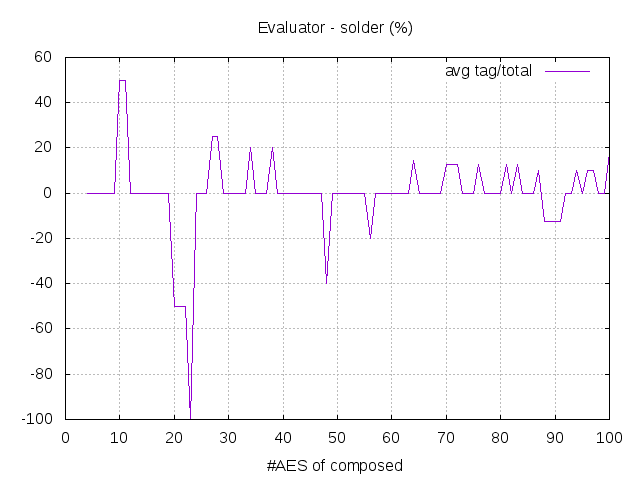
\includegraphics[width=\textwidth]{eval_solder_frac}
        \caption{Evaluator, fraction of time used on tag part}
    \end{subfigure}
    \caption{The solder phase is where the preprocessed circuits are composed into one circuit.}
    \label{data solder}
\end{figure}

\begin{figure}[h]
    \centering
    \begin{subfigure}[t]{0.3\textwidth}
        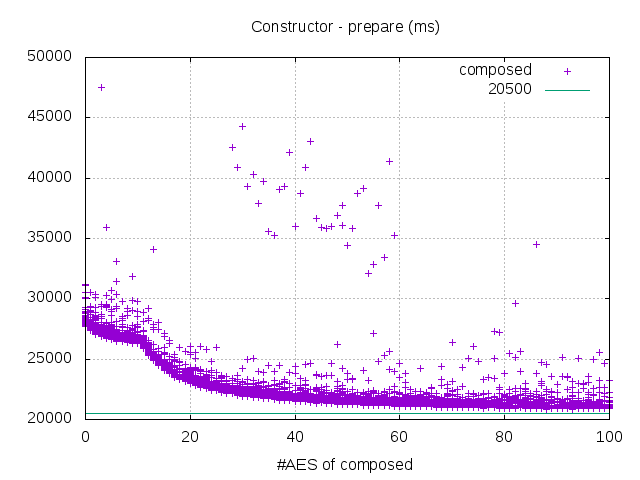
\includegraphics[width=\textwidth]{const_prepare_plots}
        \caption{Constructor, total time used on the composed circuit}
    \end{subfigure}
    \begin{subfigure}[t]{0.3\textwidth}
        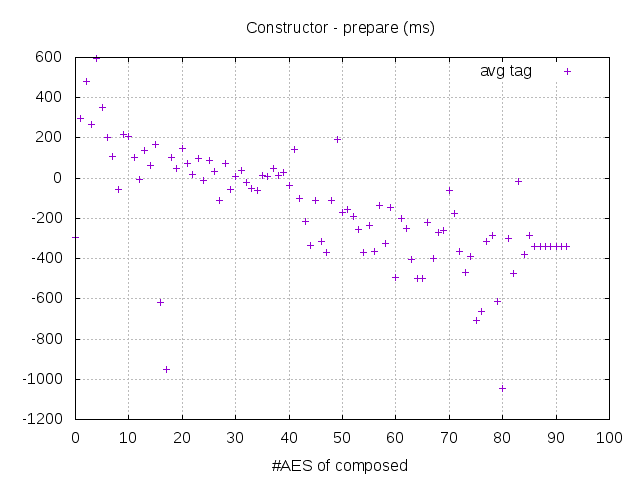
\includegraphics[width=\textwidth]{const_prepare_avg}
        \caption{Constructor, average time used on tag part}
    \end{subfigure}
    \begin{subfigure}[t]{0.3\textwidth}
        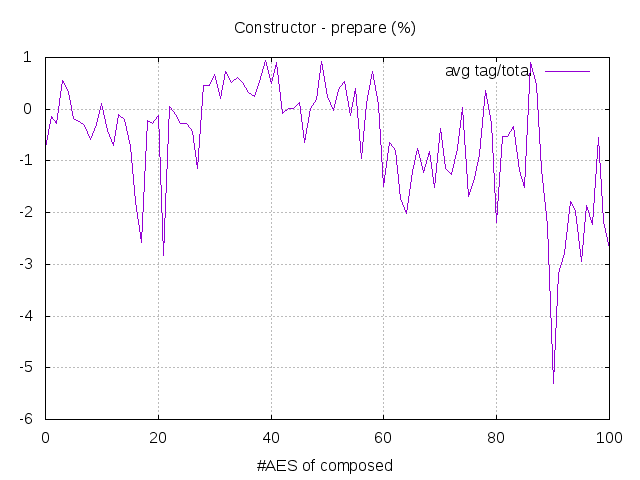
\includegraphics[width=\textwidth]{const_prepare_frac}
        \caption{Constructor, fraction of time used on tag part}
    \end{subfigure}

    \begin{subfigure}[t]{0.3\textwidth}
        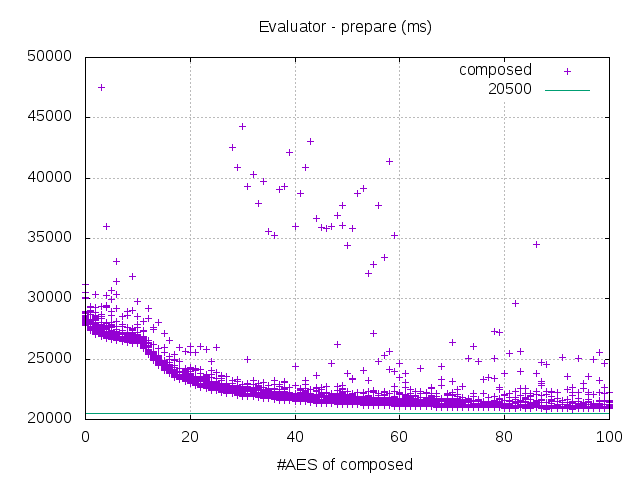
\includegraphics[width=\textwidth]{eval_prepare_plots}
        \caption{Evaluator, total time used on the composed circuit}
    \end{subfigure}
    \begin{subfigure}[t]{0.3\textwidth}
        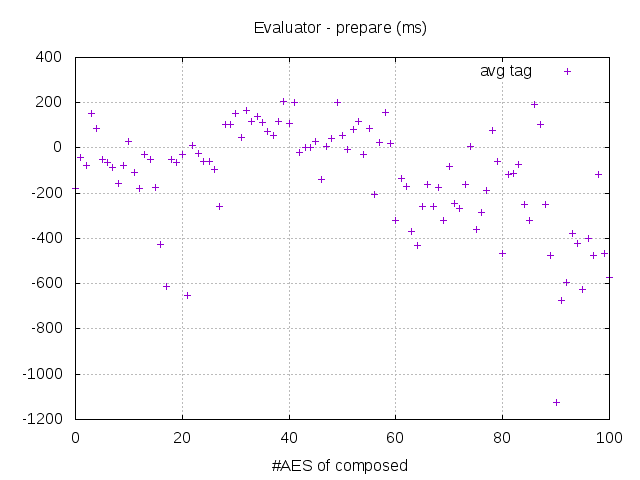
\includegraphics[width=\textwidth]{eval_prepare_avg}
        \caption{Evaluator, average time used on tag part}
    \end{subfigure}
    \begin{subfigure}[t]{0.3\textwidth}
        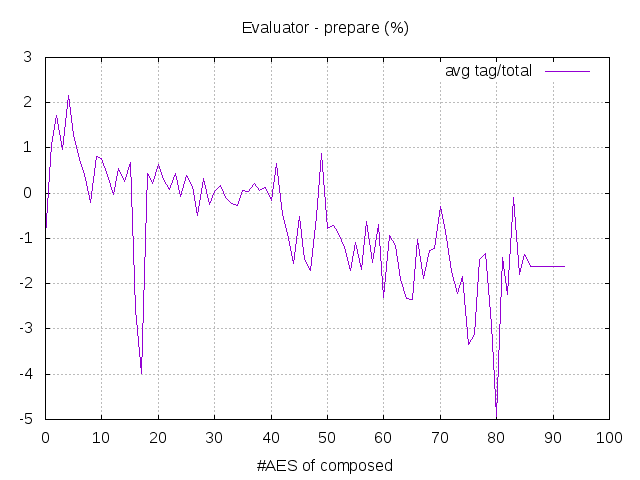
\includegraphics[width=\textwidth]{eval_prepare_frac}
        \caption{Evaluator, fraction of time used on tag part}
    \end{subfigure}
    \caption{In the prepare phase the composed circuit is prepared for evaluation.}
    \label{data prepare}
\end{figure}

\begin{figure}[h]
    \centering
    \begin{subfigure}[t]{0.3\textwidth}
        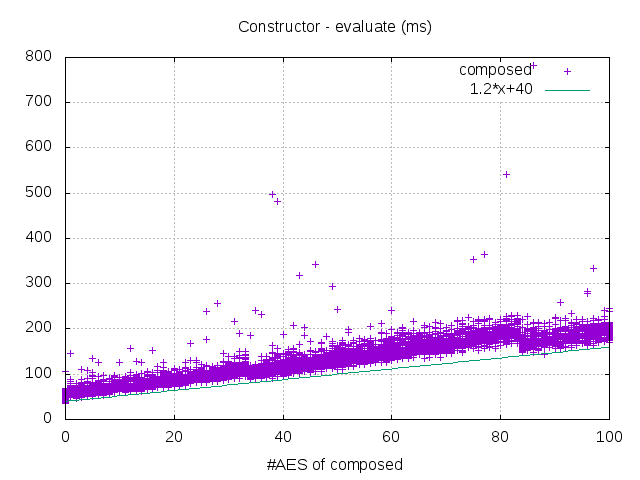
\includegraphics[width=\textwidth]{const_eval_plots}
        \caption{Constructor, total time used on the composed circuit}
    \end{subfigure}
    \begin{subfigure}[t]{0.3\textwidth}
        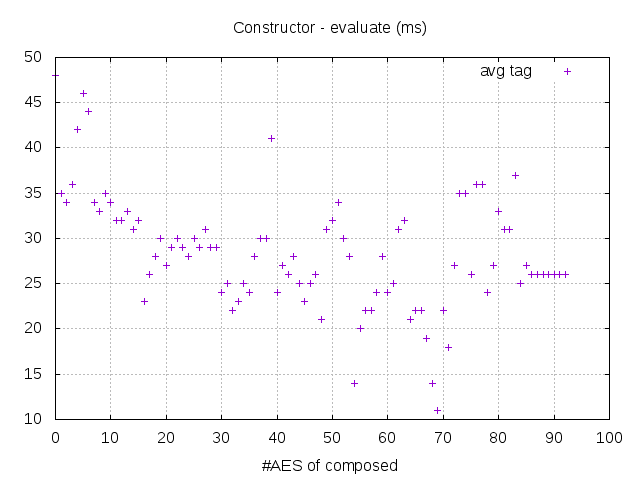
\includegraphics[width=\textwidth]{const_eval_avg}
        \caption{Constructor, average time used on tag part}
    \end{subfigure}
    \begin{subfigure}[t]{0.3\textwidth}
        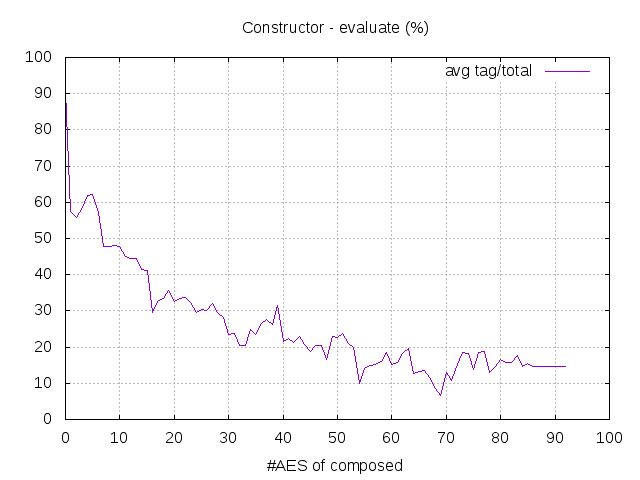
\includegraphics[width=\textwidth]{const_eval_frac}
        \caption{Constructor, fraction of time used on tag part}
    \end{subfigure}

    \begin{subfigure}[t]{0.3\textwidth}
        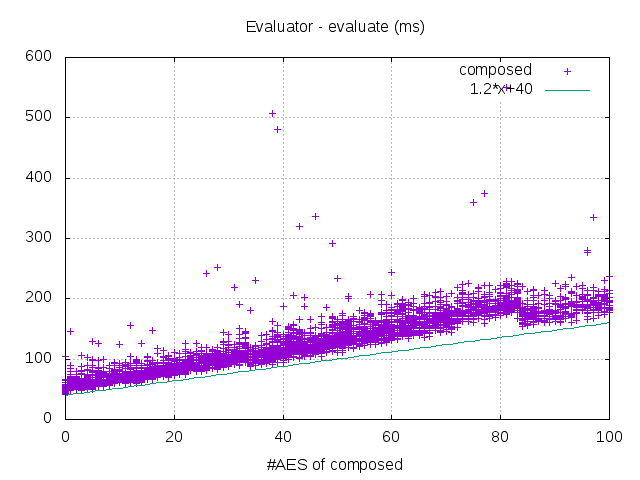
\includegraphics[width=\textwidth]{eval_eval_plots}
        \caption{Evaluator, total time used on the composed circuit}
    \end{subfigure}
    \begin{subfigure}[t]{0.3\textwidth}
        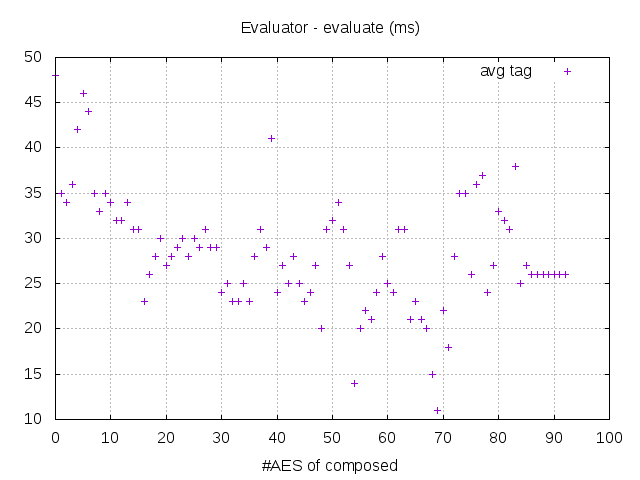
\includegraphics[width=\textwidth]{eval_eval_avg}
        \caption{Evaluator, average time used on tag part}
    \end{subfigure}
    \begin{subfigure}[t]{0.3\textwidth}
        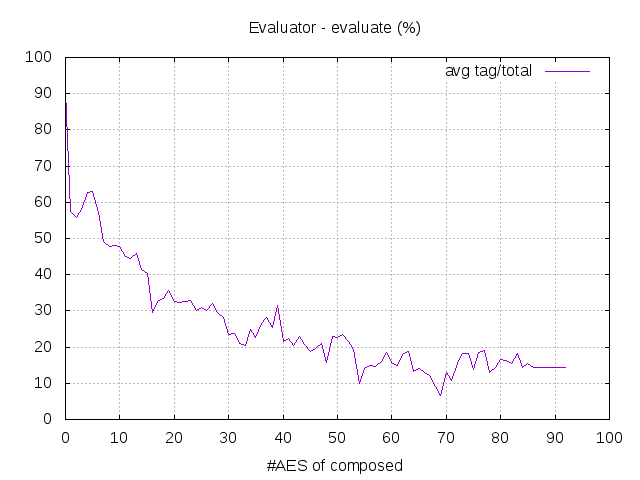
\includegraphics[width=\textwidth]{eval_eval_frac}
        \caption{Evaluator, fraction of time used on tag part}
    \end{subfigure}
    \caption{In the evaluation phase the composed circuit is evaluated.}
    \label{data evaluation}
\end{figure}

\begin{figure}[h]
    \centering
    \begin{subfigure}[t]{0.3\textwidth}
        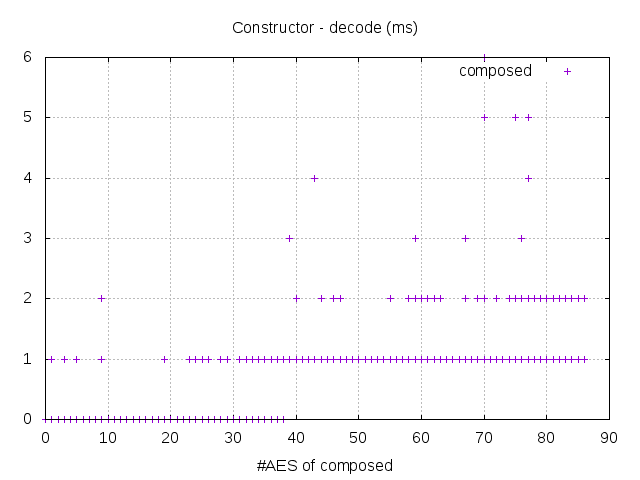
\includegraphics[width=\textwidth]{const_decode_plots}
        \caption{Constructor, total time used on the composed circuit}
    \end{subfigure}
    \begin{subfigure}[t]{0.3\textwidth}
        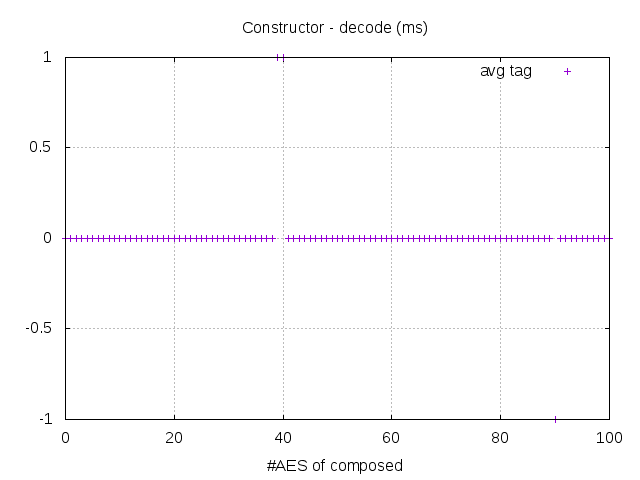
\includegraphics[width=\textwidth]{const_decode_avg}
        \caption{Constructor, average time used on tag part}
    \end{subfigure}
    \begin{subfigure}[t]{0.3\textwidth}
        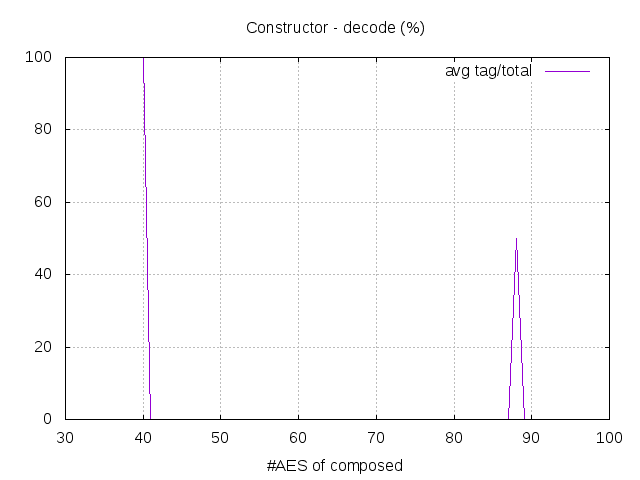
\includegraphics[width=\textwidth]{const_decode_frac}
        \caption{Constructor, fraction of time used on tag part}
    \end{subfigure}

    \begin{subfigure}[t]{0.3\textwidth}
        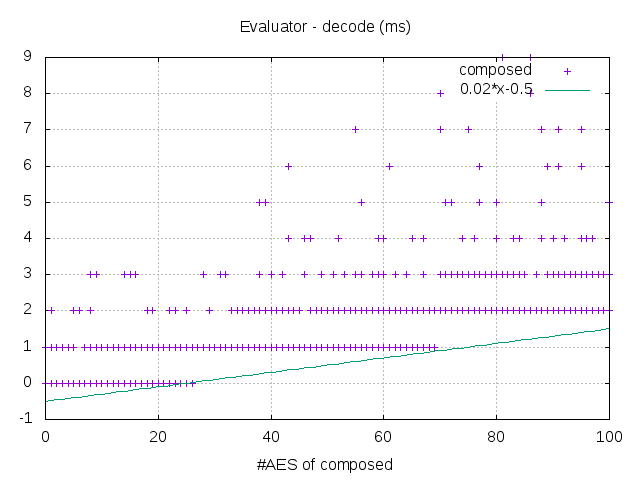
\includegraphics[width=\textwidth]{eval_decode_plots}
        \caption{Evaluator,  total time used on the composed circuit}
    \end{subfigure}
    \begin{subfigure}[t]{0.3\textwidth}
        \includegraphics[width=\textwidth]{eval_decode_avg}
        \caption{Evaluator, average time used on tag part}
    \end{subfigure}
    \begin{subfigure}[t]{0.3\textwidth}
        \includegraphics[width=\textwidth]{eval_decode_frac}
        \caption{Evaluator, fraction of time used on tag part}
    \end{subfigure}
    \caption{In the decode phase the output from the composed circuit is decoded.}
    \label{data decode}
\end{figure}

\begin{figure}[h]
    \centering
    \includegraphics[width=0.5\textwidth]{total_frac}
    \caption{For the plot every line in the composed timings has been summed and a constant upper bound for all the average plots has been used to calculate the fraction. Resulting in $\frac{300}{36x+22500}$ as an upperbound on the tag fraction of the composed circuit.}
    \label{data total}
\end{figure}

\end{document}